\documentclass[citestyle=gb7714-2015, bibstyle=gb7714-2015,lang=cn,14pt,scheme=chinese]{elegantbook}

\title{深度学习模型的学习动态}
\subtitle{xxxxx}

\author{姜广琛}
\institute{西北工业大学}
\date{2025/04/17}
\version{0.1}
% \bioinfo{自定义}{信息}

% \extrainfo{注意:本模板自 2023 年 1 月 1 日开始,不再更新和维护!}

\setcounter{tocdepth}{3}

\logo{logo-blue.png}
\cover{cover.jpg}

% 本文档命令
\usepackage{minted}
\usepackage[linesnumbered,ruled,vlined]{algorithm2e}


% 修改标题页的橙色带
\definecolor{customcolor}{RGB}{32,178,170}
\colorlet{coverlinecolor}{customcolor}
\usepackage{cprotect}

\addbibresource[location=local]{reference.bib} % 参考文献,不要删除
\ExecuteBibliographyOptions{sorting=ynt}

\begin{document}

% \maketitle
\frontmatter

\tableofcontents

\mainmatter%

\chapter{环境设置}

\section{扫地机器人(Sweeping Robot)}

对于扫地机器人的环境,我参考的是课堂 PPT 中的设置,具体环境特征概括可参考下面:

\begin{definition*}{环境描述}
\# 问题描述

    设计一个扫地机器人环境,模拟机器人在 \(5 \times 5\) 的离散网格中进行自主清扫与充电的任务。该环境共有 \(5 \times 5 = 25\) 个格子,构成了机器人的观测空间。机器人(Agent)是主要的控制对象,能够在这些格子之间进行移动。为了增加任务的复杂性和趣味性,环境中还包含了多个元素,包括垃圾、充电桩和障碍物,每个元素的设置都会影响机器人的行为决策。

\# 在这个环境中有以下组成部分:
    \begin{itemize}
        \item 垃圾 (Trash): 位于网格的 \(\left( 5, 4 \right)\)(索引从 \(1\) 开始)。当机器人到达这个位置时,获得 \(+5\) 奖励,回合结束。
        \item 充电桩 (Charger): 位于网格的 (索引从 \(1\) 开始)。当机器人到达这个位置时,获得 \(+1\) 奖励,回合结束。
        \item 障碍物 (Obstacle): 位于网格的 \(\left( 3, 3 \right)\)(索引从 \(1\) 开始)。机器人无法进入该格子。
    \end{itemize}

\# 这个环境中有以下限制:
\begin{itemize}
    \item 网格大小为 \(5 \times 5 = 25\),机器人只能在该网格内移动。
    \item 在每回合,机器人随机出生在 \(5 \times 5 = 25\) 的网格内的任意一空白随机点。
    \item 机器人每次可以选择向上、下、左或右移动一个格子。
    \item 对于障碍物所在的位置,机器人无法进入该位置。
    \item 每当机器人到达垃圾或充电桩时,回合结束。
\end{itemize}
\end{definition*}

我们主要以扫地机器人为主要例子,展示如何使用 Gymnasium 来构建我们自己的环境。

\subsection{创建环境}

首先,我们要分析需求,并使用 Gymnasium 创建我们的自定义扫地机器人环境。
对于相关具体教程,请主要参阅 \href{https://gymnasium.farama.org/introduction/create_custom_env/}{https://gymnasium.farama.org/introduction/create\_custom\_env/}。
我们先继承 \href{https://gymnasium.farama.org/api/env/#gymnasium.Env}{\textsf{gymnasium.Env}} 类来构建我们的环境:
\begin{minted}[fontsize=\small, breaklines]{python}
class SweepingRobotEnv(gym.Env):
    ...
\end{minted}

我们需要主要关注的 API 方法是:
\begin{itemize}
    \item \textsf{step()}:使用指定的动作更新环境,返回下一步代理的观测值、采取该动作所获得的奖励、环境是否因该动作而终止或截断的标志,以及来自环境的其他信息(如评估指标、调试信息)。
    \item \textsf{reset()}:将环境重置为初始状态,必须在调用 \textsf{reset()} 之前执行。返回该轮训练的第一个代理观测值以及相关信息(如评估指标、调试信息)。
    \item \textsf{render()}:渲染环境,帮助可视化代理所看到的内容。常用的渲染模式包括:“human”(人类可视)、“rgb\_array”(RGB 数组)、“ansi”(文本形式)。对于这部分,不是我们需要关注的主要内容。
    \item \textsf{close()}:关闭环境,尤其在使用外部软件(如 pygame 进行渲染,或数据库操作)时十分重要。
\end{itemize}

\subsubsection{\textsf{\_\_init\_\_} 函数中定义基本环境}

对于 \textbf{状态空间},我们可以知道智能体所处的环境是一个 \(5 \times 5\) 的格子环境,也就是一个离散空间,所以我们对于环境的建模应该使用 \href{https://gymnasium.farama.org/api/spaces/fundamental/#gymnasium.spaces.Discrete}{\textsf{spaces.Discrete}} 来构建一个 \(5 \times 5\) 的观测空间。
\textsf{spaces.Discrete} 定义了一个由整数组成的有限个元素组成的子集空间,我们主要使用它的 \texttt{n}、\texttt{start} 这两个属性,我们通过设置这两个属性,可以得到 \(\left\{ \mathtt{a}, \mathtt{a+1}, \dots, \mathtt{a+n-1} \right\}\) 这样一个有限的整数集合。而 \texttt{start} 属性默认为 \(0\)。
但是我们使用 \textsf{spaces.Discrete} 只能构建类似“一维空间”,没有办法直接定义这个 \(5 \times 5\) 的格子,即我们只能定义:
\begin{minted}[fontsize=\small, breaklines]{python}
spaces.Discrete(5)
\end{minted}

所以我们有两种解决办法,第一种是直接构建一个大小为 \(25\) 的“一维向量空间”,但我个人觉得这种办法不利于我们后续编程,会让简单的问题变得麻烦起来。
第二种方法是将两个 \(5\) 个大小的空间做笛卡尔积,来实现 \(\left(\texttt{x}, \texttt{y}\right)\) 这样的二维空间。
对于这个环境的空间,我们选择使用 \href{https://gymnasium.farama.org/api/spaces/composite/#gymnasium.spaces.Tuple}{\textsf{spaces.Tuple}} 方法将两个一维离散空间组合起来:
\begin{minted}[fontsize=\small, breaklines]{python}
self.observation_space = spaces.Tuple(
        (spaces.Discrete(size), spaces.Discrete(size))
    )
\end{minted}
当然,{\textsf{spaces.Tuple}} 方法也可以链接任意多个任意个不同的空间,例如:
\begin{minted}[fontsize=\small, breaklines]{python}
Tuple((Discrete(2), Box(-1, 1, shape=(2,))))
\end{minted}
就是将一个 \(\left\{ \mathtt{0}, \mathtt{1} \right\}\) 的整数离散空间和 使用 \href{https://gymnasium.farama.org/api/spaces/fundamental/#gymnasium.spaces.Box}{\textsf{spaces.Box}} 方法构造的 \(\left[ -1, 1 \right]\) 这个区间的连续空间结合起来。

对于 \textbf{动作空间},我们可以简单的知道,智能体可以上下左右进行移动,所以我们可以简单的通过 
\begin{minted}[fontsize=\small, breaklines]{python}
spaces.Discrete(4)
\end{minted}
来构建智能体的动作空间。

而且我们可以直接通过定义空间位置,使用一个二维数组记录 \(\left( \texttt{x}, \texttt{y} \right)\) 坐标描绘垃圾、充电桩和障碍物的位置。
\begin{minted}[fontsize=\small, breaklines]{python}
self._trash_location = np.array([3, 4])
self._charging_station_location = np.array([0, 0])
self._obstacle_location = np.array([2, 2])
\end{minted}

\subsubsection{\textsf{reset} 函数将环境设定为初始化场景}

这部分具体可以参考 \href{https://gymnasium.farama.org/api/env/#gymnasium.Env.reset}{\textsf{Env.reset}}。
通常,对于环境的 \textsf{reset} 函数,都是具有一定的随机性,所以这里我们设定 智能体 的位置可能是在这个格子空间中的除垃圾、充电桩和障碍物的任意一个格子。
这里的逻辑较为简单,可以直接看最终实现代码中的 \textsf{reset} 函数部分参考。

\subsubsection{\textsf{step} 函数定义智能体操作执行一次动作之后环境的反应}

这部分具体可以参考 \href{https://gymnasium.farama.org/api/env/#gymnasium.Env.step}{\textsf{Env.step}}。

只是在这里需要注意的是,我们需要保证当智能体行动合法,即只能在环境的限制范围内移动。
这一方法会返回几个值:
\begin{itemize}
    \item observation:环境的 observation\_space 中的一个元素,表示由于代理执行动作后获得的下一步观测值。例如,在 CartPole 环境中,这可能是一个包含杆子位置和速度的 numpy 数组。在我们这个扫地机器人的环境,我们先简单假设这里返回扫地机器人的位置信息,一个简单的 numpy 数组。
    \item reward:依据上述的环境描述,垃圾位置的收益为 \(+5\),充电桩的收益为 \(+1\),其他位置的收益都是 \(0\)。
    \item terminated:表示代理是否到达了任务马尔可夫决策过程(MDP)中定义的终止状态,该状态可以是正面或负面的。例如,到达目标状态,或在 Sutton 和 Barto 的网格世界中掉入熔岩。如果为 True,则用户需要调用 \textsf{reset}。
    \item truncated:表示是否满足了 MDP 范畴之外的截断条件。通常这是时间限制(达到最大步数),但也可以用于指智能体越界等情况。该标志可用于在尚未达到终止状态前提前结束当前回合。如果为 True,则用户需要调用 \textsf{reset}。
\end{itemize}
其他信息,例如 info 和 done,不是我们考虑的重点,并且其中 done 返回值已经被弃用,感兴趣的同学请参考官方文档。

\subsection{可视化展示}

我们的环境也做了一个简单的可视化(如图~\ref{fig:sweeping-robot-env-render}),具体代码实现需要参考代码中的 \textsf{render} 函数。

\begin{figure}[htb]
\centering
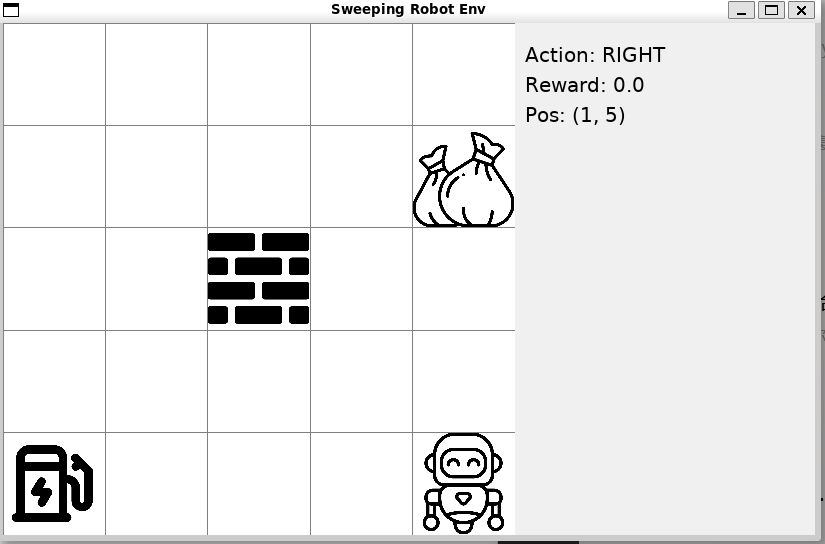
\includegraphics[width=0.48\linewidth]{image/sweep_robot_env_render1.jpg}
\hfill
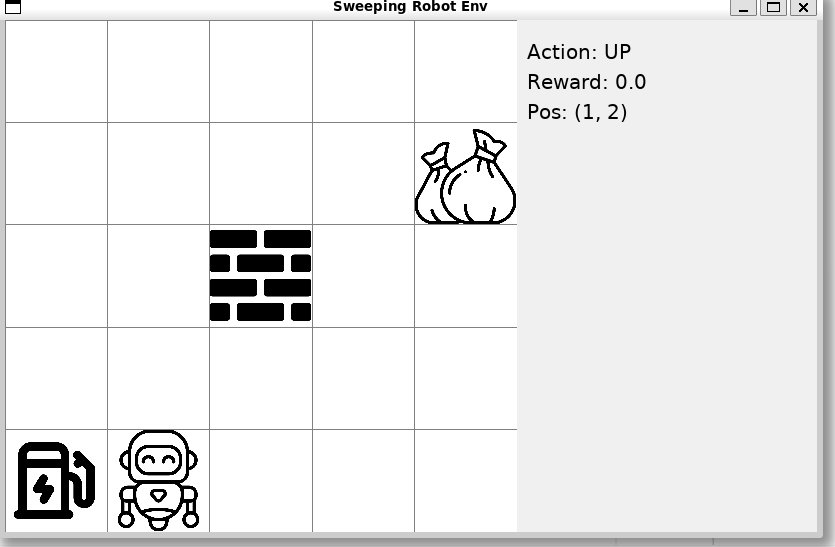
\includegraphics[width=0.48\linewidth]{image/sweep_robot_env_render2.jpg}
\caption{扫地机器人学习过程可视化展示(\textsf{render} 函数实现)}\label{fig:sweeping-robot-env-render}
\end{figure}

\subsection{具体代码}

对于扫地机器人的环境的具体代码,请参考附录~\ref{sec:sweeping-robot-env}


\section{多开关匹配}

多开关匹配是我发明的一个简单的强化学习环境,其主要的环境描写如下:

\begin{definition*}{环境描述}
\# 问题描述

    设计一个多开关匹配的强化学习环境。在该环境中,智能体的任务是通过一系列操作将开关的状态调整到目标状态。每个开关有两个可能的状态:开 (\(1\)) 或关 (\(0\))。智能体可以独立地控制每个开关的状态,置 \(1\) 代表拨动开关,置 \(0\) 代表不对开关进行操作。智能体的目标是通过最少的步骤将所有开关的状态与目标状态一致。
\end{definition*}

\subsection{使用 \textsf{spaces.MultiBinary} 构建组合构建的观测空间和动作空间}

对于这个环境,假设我们需要同时操作 \(3\) 个动作,我们需要注意的是如何构建多个动作空间构成的环境。
在这里,我们直接使用 \textsf{spaces.MultiBinary},并且官方给了一个例子。
\begin{minted}[fontsize=\small, breaklines]{python}
>>> from gymnasium.spaces import MultiBinary
>>> observation_space = MultiBinary(5, seed=42)
>>> observation_space.sample()
>>> array([1, 0, 1, 0, 1], dtype=int8)
>>> observation_space = MultiBinary([3, 2], seed=42)
>>> observation_space.sample()
>>> array([[1, 0],
           [1, 0],
           [1, 1]], dtype=int8)
\end{minted}
我们只要通过其中一个参数的大小,就可以控制这个二进制空间了。
假定我们的开关一共有 \texttt{num\_switches} 个,所以:
\begin{minted}[fontsize=\small, breaklines]{python}
self.observation_space = spaces.MultiBinary(num_switches)
self.action_space = spaces.MultiBinary(num_switches)
\end{minted}
并且通过随机设置一个目标状态,来构建我们的目标:
\begin{minted}[fontsize=\small, breaklines]{python}
self.target_state = np.random.randint(0, 2, size=num_switches)
\end{minted}
对于动作,通过 \(1\) 表示拨动开关,\(0\) 表示不拨动开关,这个在 \textsf{step} 函数中的核心逻辑为:
\begin{minted}[fontsize=\small, breaklines]{python}
self.target_state = np.random.randint(0, 2, size=num_switches)
self.state = (self.state + action) % 2
\end{minted}

\subsection{可视化展示}

我们的环境也做了一个简单的可视化(如图~\ref{fig:multiswitch-env-render}),具体代码实现需要参考代码中的 \textsf{render} 函数。

\begin{figure}[H]
    \centering
    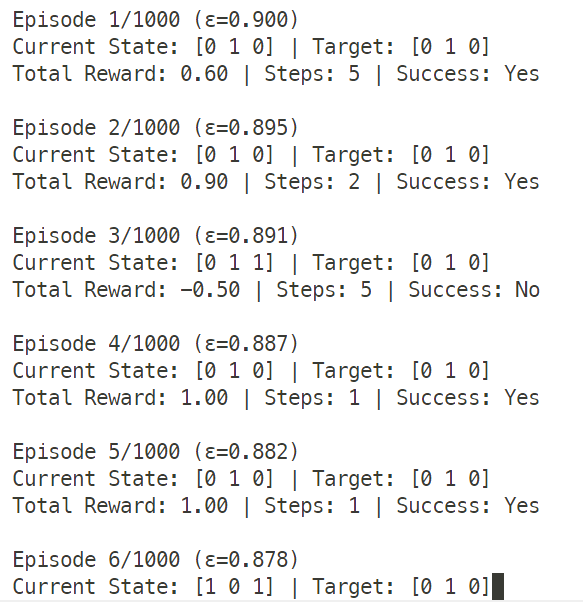
\includegraphics[width=0.5\textwidth]{image/multi-switch-env_render1.jpg}
    \caption{扫地机器人学习过程可视化展示(\textsf{render} 函数实现)}\label{fig:multiswitch-env-render}
\end{figure}

\subsection{实现代码}

对于多开关匹配的环境的具体代码,请参考附录~\ref{sec:multi-switch-env}。

\section{Double Mountain Car}

对于我创建的 Double Mountain Car 环境,是仿造经典的离散动作版本的 MountainCar 问题的扩展版本,具体代码可以参考 \href{https://gymnasium.farama.org/environments/classic_control/mountain_car}{https://gymnasium.farama.org/environments/classic\_control/mountain\_car}。
其环境的详细描述如下:

\begin{definition*}{环境描述}
\# 问题描述

    设计一个包含 两个山地车 的强化学习环境。该环境是经典离散动作的 MountainCar 问题的扩展版本~\footnote{如果你不熟悉 MountainCar 问题,请参考 \href{https://gymnasium.farama.org/environments/classic_control/mountain_car}{https://gymnasium.farama.org/environments/classic\_control/mountain\_car}。},两个智能体(小车)必须协作,利用加速度在重力势能影响下成功爬坡,到达目标位置。两个小车可以分别独立控制,它们的任务是同时达到终点位置的目标状态,回合才会终止。这个问题与 MountainCar 问题几乎一致,但是可以帮助大家熟悉 gymnasium 库中的 \href{https://gymnasium.farama.org/api/spaces/fundamental/#gymnasium.spaces.Box}{spaces.Box} 和 \href{https://gymnasium.farama.org/api/spaces/fundamental/#gymnasium.spaces.MultiDiscrete}{spaces.MultiDiscrete} 这两个基础空间类。

\# 具体要求

对于这个问题的相关具体要求,可以仔细阅读并参考 MountainCar 问题的源代码 \href{https://github.com/Farama-Foundation/Gymnasium/blob/main/gymnasium/envs/classic_control/mountain_car.py}{gymnasium/envs/classic\_control/mountain\_car.py}。
我们唯一需要做的事情就是将原本单个 Car 的状态空间与动作空间变成 两个 Car 的状态与动作空间。
熟悉相关基础类,并初步入门多智能体控制。
\end{definition*}

在此基础上,我舍弃了使用 \textsf{render} 进行可视化,而是使用 \textsf{spaces.Box} 构建小车的观测环境和使用 \href{https://gymnasium.farama.org/api/spaces/fundamental/#gymnasium.spaces.MultiDiscrete}{\textsf{spaces.MultiDiscrete}} 来构建里两个小车的联合动作。
对于 \textsf{spaces.MultiDiscrete} 的使用,与 \textsf{spaces.MultiBinary} 类似,只是参数变成了 \textsf{np.array}。
例如对于任天堂游戏手柄,可以离散化成 \(3\) 个离散的动作空间:
\begin{itemize}
    \item 方向键:\(5\) 个离散的元素 - NOOP [0]、上 [1]、右 [2]、下 [3]、左 [4] - 参数:最小值:\(0\),最大值:\(4\)。
    \item 按钮 A:\(2\) 个离散的元素 - NOOP [0],按下 [1] - 参数:最小值:\(0\),最大值:\(1\)。
    \item 按钮 B:\(2\) 个离散的元素 - NOOP [0],按下 [1] - 参数:最小值:\(0\),最大值:\(1\)。
\end{itemize}
对应的空间代码为
\begin{minted}[fontsize=\small, breaklines]{python}
spaces.MultiDiscrete([ 5, 2, 2 ])
\end{minted}


而在我们的环境中,对应的是两个小车,各 \(3\) 个动作,而环境可以被视为一个简单的 \(4\)-维的 \textsf{spaces.Box}~\footnote{也可以通过 \textsf{spaces.Tuple} 和 \textsf{spaces.Box} 组合构建。} 所以动作和环境的初始化如下:
\begin{minted}[fontsize=\small, breaklines]{python}

...
# State bounds for both cars
self.low = np.array(
    [
        self.min_position,
        -self.max_speed,  # Car 1
        self.min_position,
        -self.max_speed,  # Car 2
    ],
    dtype=np.float32,
)

self.high = np.array(
    [
        self.max_position,
        self.max_speed,  # Car 1
        self.max_position,
        self.max_speed,  # Car 2
    ],
    dtype=np.float32,
)
...
self.action_space = spaces.MultiDiscrete([3, 3])
self.observation_space = spaces.Box(self.low, self.high, dtype=np.float32)
...
\end{minted}
其他设置都和原始的 MountainCar 问题一致。
而对于可视化操作,这里就没有实现。

\subsection{实现代码}

对于 Double Mountain Car 问题的环境的具体代码,请参考附录~\ref{sec:double-mountain-car-env}。

\chapter{实验过程及结果}

在这一部分展示强化学习算法的实现。

\section{SARAS}

我们对于扫地机器人问题,首先实现了 SARSA (State-Action-Reward-State-Action) 算法。
SARSA 是一种基于时间差分(Temporal Difference, TD)的强化学习算法,用于在智能体与环境交互过程中,学习一个状态-动作价值函数(\(Q\) 函数)。它是一个 \textbf{on-policy(依策略)} 的算法,意味着它学习的是当前行为策略下的 \(Q\) 值。

SARSA 的名字来自它更新公式中用到的五个元素:
\begin{itemize}
    \item \(S_t\):当前状态(State)
    \item \(A_t\):当前动作(Action)
    \item \(R_{t+1}\):执行动作后的即时奖励(Reward)
    \item \(S_{t+1}\):下一个状态(State)
    \item \(A_{t+1}\):在下一个状态选择的动作(Action)
\end{itemize}

SARSA 的基本更新公式为:
\[
    Q^{\texttt{new}} \left( s_t, a_t \right) \leftarrow  Q \left( s_t, a_t \right) + \alpha \left[ r_{t} + \gamma Q \left( s_{t+1}, a_{t+1} - Q \left( s_t, a_t \right) \right) \right]
\]
其中,\(\alpha\) 是学习率(learning rate),\(\gamma\) 是折扣因子(discount factor),衡量未来奖励的重要性。\(Q \left( S_t, A_t \right)\) 是状态-动作价值函数。

\begin{algorithm}[H]
\caption{SARSA 算法}
\KwIn{学习率 \(\alpha\),折扣因子 \(\gamma\),探索率 \(\epsilon\)}
\KwOut{动作-状态值函数 $Q(s,a)$}

任意初始化 \(Q(s,a)\)\;

\ForEach{每一轮训练(episode)}{
    初始化状态 \(S_t\)\;
    根据当前策略从状态 \(s_t\) 中选择动作 \(a_t\)(例如 \(\epsilon\)-贪婪)\;
    \While{状态 \(s_t\) 不是终止状态}{
        执行动作 \(a_t\),观察奖励 \(r_t\) 和下一个状态 \(s_{t+1}\)\;
        从状态 \(s_{t+1}\) 根据当前策略选择动作 \(a_{t+1}\)(例如 $\epsilon$-贪婪)\;
        更新 \(Q^{\texttt{new}} \left( s_t, a_t \right) \leftarrow  Q \left( s_t, a_t \right) + \alpha \left[ r_{t} + \gamma Q \left( s_{t+1}, a_{t+1} - Q \left( s_t, a_t \right) \right) \right]\)\;
        将 \(s_t \leftarrow s_{t+1}\),\(a_t \leftarrow a_{t+1}\)\;
    }
}
\end{algorithm}

\section{Policy Gradient}

\section{\(Q\)-Learning}

\section{PPO}



\nocite{*}

\printbibliography[heading=bibintoc, title=\ebibname]
\appendix

\chapter{appendix}

\section{扫地机器人环境代码}\label{sec:sweeping-robot-env}

在这部分,展示我实现的扫地机器人的环境代码,代码接口符合 Gymnasium 的标准。

\begin{minted}[frame=single, fontsize=\small, linenos, breaklines]{python}
import gymnasium as gym
import numpy as np
import pygame
from gymnasium import spaces


class SweepingRobotEnv(gym.Env):
    metadata = {"render_modes": ["human", "rgb_array"], "render_fps": 15}

    def __init__(self, render_mode=None, size=5):
        super().__init__()
        self.size = size
        self.window_size = 512

        # 定义状态空间,在这里状态空间等同于观测空间
        self.observation_space = spaces.Tuple(
            (spaces.Discrete(size), spaces.Discrete(size))
        )
        # 定义动作空间
        self.action_space = spaces.Discrete(4)

        # 设置 agent 的默认位置
        self._agent_default_location = np.array([0, 1])
        # 记录机器人的位置,在后续的 reset 方法中会被初始化,并在 step 方法中更新
        # 此处仅仅是一个占位符,或者是冷启动状态
        self._agent_location = np.array([0, 0])
        # 垃圾、充电桩和障碍物的位置
        self._trash_location = np.array([3, 4])
        self._charging_station_location = np.array([0, 0])
        self._obstacle_location = np.array([2, 2])

        assert render_mode is None or render_mode in self.metadata["render_modes"]
        self.render_mode = render_mode

        self.window = None
        self.clock = None

        self.icons = {}

        def load_icon(name, file):
            img = pygame.image.load(file)
            img = pygame.transform.scale(
                img,
                (int(self.window_size / self.size), int(self.window_size / self.size)),
            )
            self.icons[name] = img

        load_icon("robot", "icons/robot.png")
        load_icon("trash", "icons/trash.png")
        load_icon("charger", "icons/charger.png")
        load_icon("obstacle", "icons/block.png")

    def _get_obs(self):
        """返回当前 agent 的位置

        Returns:
            tuple: 当前 agent 的位置
        """
        return tuple(self._agent_location)

    def _get_info(self):
        """返回当前 agent 的位置与垃圾和充电桩的欧几里得距离信息

        Returns:
            list: 当前 agent 的位置与垃圾和充电桩的欧几里得距离信息
        """
        return {
            "distance_to_trash": np.sum(
                np.abs(self._agent_location - self._trash_location)
            ),
            "distance_to_charger": np.sum(
                np.abs(self._agent_location - self._charging_station_location)
            ),
        }

    def reset(self, init_pos=None, seed=None, options=None):
        # 处理 Gymnasium 内部的种子等
        super().reset(seed=seed)

        # 1. 确定所有可能的有效初始位置
        initial_positions = []
        for r in range(self.size):
            for c in range(self.size):
                pos = np.array([r, c])
                if (
                    not np.array_equal(pos, self._obstacle_location)
                    and not np.array_equal(pos, self._trash_location)
                    and not np.array_equal(pos, self._charging_station_location)
                ):
                    initial_positions.append(pos)

        # 2. 从有效位置中随机选择一个
        if not initial_positions:  # 如果没有有效位置(例如网格太小或特殊点太多)
            # 设置一个备用/默认的初始位置,确保它不是充电桩或垃圾
            # (这里的逻辑可以根据具体需求调整,例如抛出错误或选择一个尽可能安全的位置)
            if (
                not np.array_equal(
                    self._agent_default_location, self._charging_station_location
                )
                and not np.array_equal(
                    self._agent_default_location, self._trash_location
                )
                and not np.array_equal(
                    self._agent_default_location, self._obstacle_location
                )
            ):
                self._agent_location = self._agent_default_location
        else:  # 如果有有效位置,那么就从有效位置中随机选择一个初始位置
            # self.np_random 是由 super().reset(seed=seed) 设置的随机数生成器
            # 它保证了如果设置了种子,随机选择是可复现的
            idx = self.np_random.integers(0, len(initial_positions))
            self._agent_location = initial_positions[idx]

        observation = self._get_obs()
        info = self._get_info()

        # 对于 RecordVideo,不需要在 reset 时调用 _render_frame
        if self.render_mode == "human":
            self._render_frame()
        elif self.render_mode == "rgb_array":
            pass

        return observation, info

    def step(self, action):
        reward = 0.0  # 默认奖励,避免未赋值情况

        direction_vectors = {
            0: np.array([-1, 0]),  # 上
            1: np.array([1, 0]),  # 下
            2: np.array([0, -1]),  # 左
            3: np.array([0, 1]),  # 右
        }
        previous_location = np.copy(self._agent_location)
        self._agent_location = self._agent_location + direction_vectors[action]
        # 限定元素在 [0, size-1] 范围内
        self._agent_location = np.clip(self._agent_location, 0, self.size - 1)

        # 遇到墙不能走,用之前的位置代替
        if np.array_equal(self._agent_location, self._obstacle_location):
            self._agent_location = previous_location

        # 定义终止符号
        terminated = False
        if np.array_equal(self._agent_location, self._trash_location):
            reward = 5.0
            terminated = True
        elif np.array_equal(self._agent_location, self._charging_station_location):
            reward = 1.0
            terminated = True

        # 设置截断符号
        truncated = False
        observation = self._get_obs()
        info = self._get_info()

        # 对于 RecordVideo,不需要在 step 时主动调用 _render_frame
        # RecordVideo 包装器会在需要时调用 env.render()
        if self.render_mode == "human":
            self._render_frame()

        self._last_action = action
        self._last_reward = reward

        return observation, reward, terminated, truncated, info

    def render(self):
        # render 方法现在必须能处理 'rgb_array' 模式并返回图像
        if self.render_mode == "rgb_array":
            return self._render_frame()
        elif self.render_mode == "human":
            self._render_frame()  #  对于 human 模式,只渲染不返回
            return None  # Human mode render typically doesn't return
        else:
            super().render()  # 或者 gym.Env.render(self)

    def _render_frame(self):
        if self.window is None and self.render_mode == "human":
            pygame.init()
            pygame.display.init()
            self.window = pygame.display.set_mode(
                (self.window_size + 300, self.window_size)
            )
            pygame.display.set_caption("Sweeping Robot Env")

        if self.clock is None and self.render_mode == "human":
            self.clock = pygame.time.Clock()

        if pygame.display.get_init() == 0:
            pygame.init()

        for event in pygame.event.get():
            if event.type == pygame.QUIT:
                pygame.quit()
                self.close()

        # 初始化字体
        if not hasattr(self, "_info_font"):
            pygame.font.init()
            self._info_font = pygame.font.SysFont("Arial", 20)

        # 创建 canvas
        canvas = pygame.Surface((self.window_size + 300, self.window_size))
        canvas.fill((255, 255, 255))
        pix_square_size = self.window_size / self.size

        # 绘制元素图标
        def draw_icon(name, pos):
            if name in self.icons:
                icon = self.icons[name]
                canvas.blit(
                    icon,
                    (
                        pos[1] * pix_square_size,
                        (self.size - 1 - pos[0]) * pix_square_size,
                    ),
                )

        draw_icon("trash", self._trash_location)
        draw_icon("charger", self._charging_station_location)
        draw_icon("obstacle", self._obstacle_location)
        draw_icon("robot", self._agent_location)

        # 绘制网格
        for x in range(self.size + 1):
            pygame.draw.line(
                canvas,
                (128, 128, 128),
                (0, pix_square_size * x),
                (self.window_size, pix_square_size * x),
                width=1,
            )
            pygame.draw.line(
                canvas,
                (128, 128, 128),
                (pix_square_size * x, 0),
                (pix_square_size * x, self.window_size),
                width=1,
            )

        # 绘制右侧信息区域背景
        pygame.draw.rect(
            canvas,
            (240, 240, 240),
            pygame.Rect(self.window_size, 0, 300, self.window_size),
        )

        # 显示 agent 状态信息
        info_lines = []
        if hasattr(self, "_last_action"):
            action_name = ["UP", "DOWN", "LEFT", "RIGHT"][self._last_action]
            info_lines.append(f"Action: {action_name}")
        if hasattr(self, "_last_reward"):
            info_lines.append(f"Reward: {self._last_reward:.1f}")
        info_lines.append(
            f"Pos: ({int(self._agent_location[0] + 1)}, {int(self._agent_location[1] + 1)})"
        )

        for i, line in enumerate(info_lines):
            text_surf = self._info_font.render(line, True, (0, 0, 0))
            canvas.blit(text_surf, (self.window_size + 10, 20 + i * 30))

        # 渲染输出
        if self.render_mode == "human":
            self.window.blit(canvas, canvas.get_rect())
            pygame.event.pump()
            pygame.display.update()
            self.clock.tick(self.metadata["render_fps"])
            return None
        elif self.render_mode == "rgb_array":
            return np.transpose(
                np.array(pygame.surfarray.pixels3d(canvas)),
                axes=(1, 0, 2),
            )

    def close(self):
        if self.window is not None:
            pygame.display.quit()
            # pygame.quit() # pygame.quit() 会卸载所有 pygame 模块,如果其他地方还需要 pygame,可能会出问题
            self.window = None
        # 确保在所有 pygame 操作完成后才调用 pygame.quit()
        # 对于 RecordVideo, 只要 display 模块关闭即可,pygame.quit()可以在程序完全结束时调用
        if pygame.get_init():  # 检查 pygame 是否已初始化
            pygame.quit()
\end{minted}

\section{多开关匹配环境代码}\label{sec:multi-switch-env}

在这部分,展示我实现的多开关匹配的环境代码,代码接口符合 Gymnasium 的标准。

\begin{minted}[frame=single, fontsize=\small, linenos, breaklines]{python}
import sys
import time

import gymnasium as gym
import numpy as np
from gymnasium import spaces


class MultiSwitchEnv(gym.Env):
    metadata = {"render_modes": ["human"], "render_fps": 10}

    def __init__(self, render_mode=None, num_switches=3):
        super().__init__()
        self.num_switches = num_switches

        # 状态空间和动作空间都是 MultiBinary: 每个开关两个状态 0/1
        self.observation_space = spaces.MultiBinary(num_switches)
        self.action_space = spaces.MultiBinary(num_switches)  # 每个开关切或不切

        self.target_state = np.random.randint(0, 2, size=num_switches)
        self.state = None
        self.render_mode = render_mode
        self.steps = 0
        self.max_steps = 5

    def reset(self, seed=None, options=None):
        super().reset(seed=seed)
        self.state = self.np_random.integers(0, 2, size=self.num_switches)
        self.steps = 0
        return self.state.copy(), {}

    def step(self, action):
        self.steps += 1

        # 应用动作: 切换值(异或操作)
        self.state = (self.state + action) % 2

        done = np.array_equal(self.state, self.target_state)
        reward = 1.0 if done else -0.1
        truncated = self.steps >= self.max_steps

        return self.state.copy(), reward, done, truncated, {}

    def render(self):
        output = f"\rCurrent State: {self.state} | Target: {self.target_state}"
        sys.stdout.write(output)
        sys.stdout.flush()
        time.sleep(0.3)

    def close(self):
        pass
\end{minted}

\section{Double Mountain Car 环境代码}\label{sec:double-mountain-car-env}

\begin{minted}[frame=single, fontsize=\small, linenos, breaklines]{python}
import math
from typing import Optional

import gymnasium as gym
import numpy as np
from gymnasium import spaces
from gymnasium.envs.classic_control import utils


class DoubleMountainCarEnv(gym.Env):
    """
    Double Mountain Car Environment - Two cars that need to cooperate to reach the goal.

    ## Description
    This is an extension of the classic Mountain Car environment with two cars.
    Each car can be controlled independently, and they need to strategically
    accelerate to reach their respective goals.

    ## Observation Space
    The observation is a `ndarray` with shape `(4,)`:
    - [0]: position of car 1
    - [1]: velocity of car 1
    - [2]: position of car 2
    - [3]: velocity of car 2

    ## Action Space
    MultiDiscrete([3, 3]) - Each car has 3 actions:
    - 0: Accelerate to the left
    - 1: Don't accelerate
    - 2: Accelerate to the right
    """

    metadata = {
        "render_modes": [],
        "render_fps": 30,
    }

    def __init__(self, render_mode: Optional[str] = None, goal_velocity: float = 0):
        # Physical parameters
        self.min_position = -1.2
        self.max_position = 0.6
        self.max_speed = 0.07
        self.goal_position = 0.5
        self.goal_velocity = goal_velocity

        self.force = 0.001
        self.gravity = 0.0025

        # State bounds for both cars
        self.low = np.array(
            [
                self.min_position,
                -self.max_speed,  # Car 1
                self.min_position,
                -self.max_speed,  # Car 2
            ],
            dtype=np.float32,
        )

        self.high = np.array(
            [
                self.max_position,
                self.max_speed,  # Car 1
                self.max_position,
                self.max_speed,  # Car 2
            ],
            dtype=np.float32,
        )

        # Rendering
        self.render_mode = render_mode
        self.screen_width = 600
        self.screen_height = 400
        self.screen = None
        self.clock = None
        self.isopen = True

        # Action and observation spaces
        self.action_space = spaces.MultiDiscrete([3, 3])
        self.observation_space = spaces.Box(self.low, self.high, dtype=np.float32)

        # Initialize state
        self.state = None

    def step(self, action: np.ndarray):
        assert self.action_space.contains(action), (
            f"{action!r} ({type(action)}) invalid"
        )

        # Extract positions and velocities
        pos1, vel1, pos2, vel2 = self.state

        # Update car 1
        vel1 += (action[0] - 1) * self.force + math.cos(3 * pos1) * (-self.gravity)
        vel1 = np.clip(vel1, -self.max_speed, self.max_speed)
        pos1 += vel1
        pos1 = np.clip(pos1, self.min_position, self.max_position)
        if pos1 == self.min_position and vel1 < 0:
            vel1 = 0

        # Update car 2
        vel2 += (action[1] - 1) * self.force + math.cos(3 * pos2) * (-self.gravity)
        vel2 = np.clip(vel2, -self.max_speed, self.max_speed)
        pos2 += vel2
        pos2 = np.clip(pos2, self.min_position, self.max_position)
        if pos2 == self.min_position and vel2 < 0:
            vel2 = 0

        # Check termination - both cars need to reach the goal
        car1_at_goal = pos1 >= self.goal_position and vel1 >= self.goal_velocity
        car2_at_goal = pos2 >= self.goal_position and vel2 >= self.goal_velocity
        terminated = bool(car1_at_goal and car2_at_goal)

        # Reward: -1 per timestep, bonus when both reach goal
        reward = -1.0
        # Update state
        self.state = np.array([pos1, vel1, pos2, vel2], dtype=np.float32)

        if self.render_mode == "human":
            self.render()

        return self.state, reward, terminated, False, {}

    def reset(
        self,
        *,
        seed: Optional[int] = None,
        options: Optional[dict] = None,
    ):
        super().reset(seed=seed)

        # Initialize both cars at random positions
        low, high = utils.maybe_parse_reset_bounds(options, -0.6, -0.4)

        # Car 1 starts at a random position
        pos1 = self.np_random.uniform(low=low, high=high)
        vel1 = 0

        # Car 2 starts at a different random position
        pos2 = self.np_random.uniform(low=low, high=high)
        vel2 = 0

        self.state = np.array([pos1, vel1, pos2, vel2], dtype=np.float32)

        if self.render_mode == "human":
            self.render()

        return self.state, {}
\end{minted}

\end{document}
